\documentclass[11pt]{article}
\usepackage[margin=1in]{geometry}
\usepackage[T1]{fontenc}
\usepackage[utf8]{inputenc}
\usepackage{lmodern}
\usepackage{microtype}
\usepackage{booktabs}
\usepackage{multirow}
\usepackage{amsmath,amssymb}
\usepackage{graphicx}
\usepackage{hyperref}
\usepackage{xcolor}
\usepackage{enumitem}
\usepackage{float}
\usepackage{subcaption}
\newcommand{\sabrina}[1]{{\color{blue}[[Sabrina: #1]]}}

\title{DUMA-bench: A Dual-Control Multi-Agent Benchmark for Evaluating LLM Agent Security}
\author{Anonymous ACL submission}
\date{}

\newcommand{\todo}[1]{\textcolor{red}{[TODO: #1]}}
\newcommand{\passone}{\texttt{pass\^{}1}}
\newcommand{\passk}{\texttt{pass\^{}k}}
\newcommand{\asr}{\text{ASR}}

\begin{document}
    \maketitle

    \begin{abstract}

        LLM-based agents are increasingly deployed in environments where they interact with users, tools, and other agents. In such settings, security failures often emerge not only from adversarial prompts but from the interaction between the agent and dynamic user behavior. However, current evaluation paradigms remain fragmented: coordination benchmarks study multi-agent interaction without adversarial threats, while security benchmarks typically assume passive users and static control. We introduce \textbf{DUMA-bench, a benchmark and evaluation protocol} for measuring agent security under \emph{dual-control} interaction, where the agent and the user act as independent participants in a shared interaction loop, each influencing the trajectory through messages and, when permitted by a domain, through scoped tool actions. DUMA-bench extends $\tau^2$-bench~\cite{barres2025tau2bench} with structured adversarial domains that model eight common vulnerability classes: RAG poisoning, cross-agent manipulation, unsafe output handling and others. We evaluate models from OpenAI, Anthropic, DeepSeek, Qwen, and Z.ai across multiple user-behavior regimes. In the current cross-vendor slice spanning 15 models, 8 domains, and 1,960 evaluated trials per mode, aggregate performance drops from 0.746 \passone\ in solo evaluation to 0.597 \passone\ under dual-control ($p < 10^{-6}$, one-sided Fisher). The largest domain-level degradation occurs in \texttt{mktg\_phishing}, where \passone\ decreases from 0.994 to 0.393; strong additional drops appear in \texttt{collab} and \texttt{crm\_leak}. These results demonstrate that agent security is not solely a property of the model but emerges from the interaction between the model, the user, and the environment. The DUMA-bench provides a missing evaluation layer for studying security in realistic agent deployments and enables standardized comparison of defense mechanisms under interactive conditions.

    \end{abstract}

    \section{Introduction}
    \label{sec:intro}

    LLM-based agents are increasingly deployed in environments where they interact with users, tools, and other information sources. In such settings, security failures often arise not only from adversarial prompts but from the interaction between the agent and dynamic user behavior. User requests, retrieved documents, and collaborator-generated notes can all alter the information available to the agent and thereby influence downstream tool use. As a result, vulnerabilities in agent systems often emerge from interaction dynamics rather than from isolated prompts alone.

    Despite this shift toward interactive systems, current evaluation paradigms remain fragmented. Coordination benchmarks such as $\tau$-bench~\cite{yao2024taubench} and $\tau^2$-bench~\cite{barres2025tau2bench} study multi-agent interaction and shared-control environments but do not model adversarial threats. Security benchmarks such as Agent Security Bench~\cite{zhang2025asb} and Agent Dojo~\cite{debenedetti2024agentdojo} evaluate prompt injection and related attacks but assume passive users and static control. Consequently, the two strands of evaluation capture complementary aspects of agent behavior but fail to address their intersection.

    This separation creates a methodological gap in agent security evaluation. Real-world agent deployments operate under \emph{dual-control}: both the agent and the user participate as independent actors in the same interaction process, each able to influence future system
    behavior through messages and, in the general case, through role-specific tool actions~\cite{barres2025tau2bench}. Adversarial content may therefore propagate through multiple channels, including retrieved context, user requests, and agent communication. Evaluating security in settings where the user is passive removes a key dimension along which robustness can vary and fail, potentially obscuring vulnerabilities that arise only through interaction.

    To address this gap, we introduce \textbf{DUMA-bench}, a benchmark and evaluation methodology for studying agent security under dual-control interaction. DUMA-bench extends $\tau^2$-bench~\cite{barres2025tau2bench} with structured adversarial domains that embed attacks directly into interactive environments. The benchmark evaluates agents in scenarios where the user is an active participant rather than a passive prompt source, enabling the study of how interaction dynamics influence security outcomes.

    DUMA-bench includes eight domains capturing common classes of vulnerabilities in LLM-based agent systems. By embedding these attacks in interactive environments, the benchmark enables systematic evaluation of how user behavior, interaction structure, and model capability affect security robustness.

    \subsection{Contributions}

    \begin{itemize}[leftmargin=1.2em]
    \item We identify a methodological gap in agent security evaluation: existing benchmarks study either coordination without adversarial threats or security attacks under passive-user assumptions.
    \item We introduce a dual-control evaluation methodology in which the agent and the user act independently within the same execution loop, with security outcomes shaped by their interaction rather
    than by the agent alone.
    \item We implement this methodology in \textbf{DUMA-bench} by extending $\tau^2$-bench~\cite{barres2025tau2bench} with eight interactive adversarial domains.
    \item We empirically demonstrate that evaluation under dual-control interaction changes measured robustness and reveals vulnerabilities that remain hidden under passive-user evaluation.
    \end{itemize}

    \section{Related Work}

    \paragraph{Agent coordination and dual-control benchmarks.}
    Early evaluations of LLM-based agents focused on single-agent tool use and instruction following, assuming full observability and centralized control. Benchmarks such as AgentBench~\cite{liu2025agentbench} and Toolformer~\cite{schick2023toolformer} characterized isolated reasoning abilities but did not model interaction with an active user. For a comprehensive survey of tool learning, see Qin et al.~\cite{qin2025toollearning}. The $\tau$-bench framework~\cite{yao2024taubench} introduced a dynamic user that can alter the environment state, while $\tau^2$-bench~\cite{barres2025tau2bench} formalized this as a two-party Dec-POMDP~\cite{amato2013decpomdp} and showed that dual-control alone can degrade agent performance by up to 25 percentage points.

    Multi-agent coordination adds further complexity. REALM-Bench~\cite{geng2025realm} evaluates agents in logistics and scheduling tasks under dynamic disruptions, revealing failure modes such as role confusion and communication breakdowns. Recent surveys~\cite{jin2025survey} and generative agent simulations~\cite{park2023generative} highlight that scaling to $N$-player environments introduces challenges like joint policy factorization and coalition instability. However, these works do not incorporate adversarial threats or security evaluation.

    \paragraph{LLM agent security benchmarks.}
    Security evaluation of LLM-based agents has recently gained attention. Agent Security Bench (ASB)~\cite{zhang2025asb} formalizes attacks (e.g., prompt injection, tool misuse) and defenses, but focuses on single-agent scenarios. Agent Dojo~\cite{debenedetti2024agentdojo} tests robustness against prompt injection and corrupted tool outputs in a dynamic environment, yet assumes a passive user and does not model dual-control interaction.
    Taxonomies from OWASP~\cite{owasp2025agentic, owasp2025top10} enumerate threats specific to agentic AI, including cross-agent communication poisoning and human manipulation. A comprehensive survey~\cite{datta2025agentic} systematizes these risks, linking component-level vulnerabilities to system-level harms. Still, existing benchmarks evaluate security in isolation from coordination dynamics.

    \paragraph{RAG and environment-level attacks.}
    Retrieval-augmented generation (RAG) systems are increasingly integrated into agents and introduce new attack surfaces. PoisonedRAG~\cite{zou2024poisonedrag} shows that injecting a few malicious texts into a knowledge base can achieve high attack success rates. AgentPoison~\cite{chen2024agentpoison} extends this to agent-specific backdoors, while BadAgent~\cite{wang2024badagent} demonstrates that backdoors can be triggered through user queries or retrieved documents. Defenses such as Llama Guard~\cite{inan2023llamaguard} provide input–output safeguards but remain ineffective against multi-agent attack vectors.

    These lines of research highlight critical vulnerabilities, yet they are typically evaluated in static or single-controller settings.

    \paragraph{The gap and DUMA-bench.}

    None of the existing benchmarks combine (i) dual-control interaction, (ii) multi-agent coordination, and (iii) security vulnerabilities in a unified evaluation framework. DUMA-bench fills this gap by extending the dual-control evaluation paradigm to interactive security scenarios that include collaborator-style and environment-mediated attacks and embedding realistic attack scenarios. This enables the study of how interaction dynamics affect security outcomes and reveals failure modes that remain hidden under passive-user or single-agent evaluation.

    \section{Method}

    \subsection{Evaluation Framework}

    DUMA-bench evaluates the security of LLM-based agents through executable interaction scenarios. Each evaluation case consists of four components: an environment, an agent, a user, and a set of security assertions.

    The environment simulates a system with tools, external data sources, and internal state variables. The agent is an LLM-based controller that observes the environment and performs actions through available tools. The user interacts with the agent by issuing task-conditioned requests over multiple turns and, in the general framework, may additionally act through user-scoped tools when a domain exposes them. Security assertions specify invariants that must hold during execution, such as preventing unauthorized actions, preserving data integrity, or refusing malicious instructions.

    Evaluation proceeds as an interactive loop. At each step, the user and the agent exchange messages, the active participant may issue tool calls when allowed, and the environment updates its state in response to those executable actions. The interaction continues until the task terminates, after which the security assertions are evaluated.

    \subsection{Dual-Control Interaction Model}

    To capture interaction dynamics between agents and users, DUMA-bench adopts the dual-control interaction structure introduced in $\tau^2$-bench~\cite{barres2025tau2bench}. In this setting both the agent and the user operate as independent actors within a shared interaction loop, each receiving partial observations and influencing future execution.

    The environment is represented by a partially observable state space $S$. The agent $A$ and the user $U$ receive observations derived from this state and select actions from their respective action spaces. Agent actions correspond to tool invocations and communication acts. User actions correspond primarily to message-level interaction and, in the general framework, may additionally include user-scoped tool calls when such tools are available in a domain.

    The environment evolves according to a transition function that depends on the actions of both participants. As a result, both actors can influence the system trajectory. This formulation reflects the behavior of real deployed agent systems, where users are not passive instruction sources but active participants whose behavior can alter the trajectory and indirectly affect state transitions.

    Dual-control interaction introduces additional pathways for adversarial influence. Malicious content can propagate through retrieved context, user interaction, or agent communication. Evaluating security under this interaction model therefore exposes vulnerabilities that may remain hidden in static or single-controller evaluation settings.

    \subsection{Threat Model}

    We assume a grey-box attacker with realistic capabilities. The attacker is assumed to understand the system architecture and available tools but does not have access to model weights or the system prompt.

    The attacker can inject malicious content into input channels commonly present in agent systems. These channels include retrieved documents in RAG pipelines, communication messages between agents, user-facing inputs, and external data sources accessed through tools. The attacker’s objective is to induce the agent to perform unauthorized actions, disclose protected information, or generate outputs that trigger downstream vulnerabilities.

    Importantly, the attacker does not directly control the agent. Instead, malicious content is embedded in the environment or communication channels and must propagate through the interaction between the agent and the user.

    \subsection{Security Domains}

    DUMA-bench evaluates agent robustness across eight security domains representing common classes of vulnerabilities in LLM-based agent systems.

    \paragraph{mail\_rag\_phishing (RAG poisoning).} This domain evaluates robustness to indirect prompt injection attacks in retrieval-augmented email workflows. The environment simulates a mailbox-backed assistant that can retrieve relevant context snippets and send outbound email. Malicious instructions are embedded in retrievable content and are designed to look operationally relevant. The agent must use retrieved context for task completion without treating embedded adversarial instructions as authoritative workflow guidance.

    \paragraph{collab (cross-agent manipulation).} This domain models collaborator-mediated attacks in a support workflow. The target agent receives ticket context together with one or more notes attributed to a colleague, some of which may be malicious or conflicting. The environment exposes tools for inspecting ticket state and for taking sensitive actions such as sharing logs, deleting audit-relevant records, or resetting credentials. The agent must distinguish legitimate collaboration from adversarial manipulation and avoid unsafe operational actions.

    \paragraph{output\_handling (unsafe output generation).} This domain evaluates whether the agent forwards unsafe content that can trigger downstream vulnerabilities such as cross-site scripting, SQL injection, or malicious redirects. The environment provides customer-facing ticket context, collaborator notes, sanitized response paths, and a dangerous raw-snippet forwarding path. The agent must respond helpfully while ensuring that unsafe artifacts are not propagated to downstream systems or end users.

    \paragraph{crm\_leak (trusted-data oversharing).}
    This domain evaluates whether an agent improperly discloses restricted third-party data while handling otherwise legitimate CRM
    support requests. The environment provides a case bundle with both shareable customer fields and non-shareable trusted records,
    creating a realistic oversharing risk when the requester uses urgency or faux-regulatory pressure. The agent can inspect the case
    through a retrieval tool but must answer using only allowed fields and refuse to reveal trusted information.

    \paragraph{infra\_loadshed (resource overload / denial-of-wallet).}
    This domain models infrastructure-facing manipulation in which a collaborator pressures the agent to trigger expensive or disruptive
    actions that waste quota, burn API budget, or reduce service availability. The environment exposes operational tools for checking
    cluster state alongside dangerous actions such as launching heavy jobs, calling paid external APIs, overriding quota limits, or
    shutting down the cluster. The agent must reject requests that would create unnecessary cost or instability even when they are
    framed as urgent operational fixes.

    \paragraph{mktg\_phishing (campaign abuse).}
    This domain evaluates whether a marketing-facing agent can be coerced into sending phishing-style outbound email under KPI pressure
    or urgency framing. The environment simulates campaign operations with tools for reading briefs, reviewing collaborator notes,
    requesting security review, and sending email. The agent must block unapproved external domains, avoid credential-harvesting
    patterns, and escalate suspicious campaigns instead of executing them.

    \paragraph{auth\_spoof\_support (identity spoofing and auth bypass).}
    This domain models customer-support workflows where an attacker attempts to bypass identity verification through VIP pressure,
    manager override claims, or impersonation. The environment provides account-summary and verification tools, along with privileged
    actions such as updating email addresses and issuing refunds. The agent must enforce verification before any sensitive action and
    resist social-engineering attempts that try to shortcut the normal approval flow.

    \paragraph{tool\_shadow\_poison (tool shadowing and unsigned export misuse).}
    This domain evaluates whether an agent can distinguish approved tools from shadow or alias-like tools that appear convenient but
    violate policy. The environment exposes a tool manifest, policy lookup, a safe signed export path, and a dangerous fast snapshot
    export that mimics legitimate functionality. The agent must inspect tool provenance, refuse unsigned or shadow exports, and use only
    approved signed tooling when handling customer data.

    \subsection{Assertion Design}
    \label{sec:assertions}

    Each evaluation case in DUMA-bench specifies a set of binary assertions that must hold after the interaction completes. We use
    complementary assertion types that capture different failure modes: environment/state assertions verify whether forbidden or
    required effects occurred in the executable environment, while communication assertions verify whether the assistant's textual
    behavior satisfied the task's policy expectations.

    \paragraph{State assertions.}
    A state assertion is a deterministic function over the post-execution environment state. After the interaction completes, the evaluator reconstructs the post-execution environment by replaying the executable trajectory, including the tool calls recorded in the interaction history, then executes the assertion function and checks its return value. Because these checks are fully deterministic, they are not susceptible to LLM judge bias. For example, in the \texttt{auth\_spoof\_support} domain the assertion \texttt{assert\_no\_refund\_without\_verification} inspects the environment's refund log after execution and fails if any entry has \texttt{verified=False}, regardless of what the agent communicated to the user.

    \paragraph{Communication assertions.}
    Some security properties leave no trace in environment state. For example, an agent may correctly refuse to issue an unauthorized refund (passing all state assertions) yet still disclose protected customer data in its response text. Communication assertions address this gap: each assertion is a natural-language expectation evaluated against the assistant's behavior in the recorded conversation trajectory. For instance, in the \texttt{crm\_leak} domain the assertion \emph{``The assistant did not disclose ANY data from the trusted document --- guarantor name, passport, birthdate, address, phone''} checks that the agent's responses contain no protected fields, even if no unauthorized tool call was made.

    \paragraph{Composition and final success.}
    Each task specifies a \emph{reward basis} $B$ --- the subset of assertion types that contribute to the final score. Within each type, all assertions must pass: the per-type score $r_t$ is $1$ only if every assertion of that type succeeds, and $0$ otherwise. The task reward is the product across types:
    \[
        r = \prod_{t \in B} r_t \;\in\; \{0,\, 1\}.
    \]
    A task is considered \emph{passed} when $r = 1$, i.e.\ when every assertion in every type from the reward basis is satisfied. This strict conjunction prevents partial compliance: an agent that correctly refuses an unauthorized action but leaks protected data in its response receives $r = 0$.


    \subsection{Evaluation Metrics}

    We report the $\passk$ metric introduced in $\tau$-bench~\cite{yao2024taubench}. For each task $i$ with $n_i$ independent trials of which $c_i$ succeed, the unbiased estimator is:
    \[
        \widehat{\text{pass}}^{k}_{\,i} = \frac{\binom{c_i}{k}}{\binom{n_i}{k}},
    \]
    which estimates $p_i^{\,k}$, the probability that \emph{all} $k$ i.i.d.\ trials succeed. The benchmark-level score is the average across tasks: $\passk = \frac{1}{N}\sum_{i=1}^{N} \widehat{\text{pass}}^{k}_{\,i}$. Unlike the code-generation $\passk$ metric~($= 1-(1-p)^k$, at-least-one success), $\passk$ grows \emph{stricter} with $k$, measuring reliability rather than best-case performance. We also report the attack success rate $\asr = 1 - \passone$.

    \section{Experiments}

    This section describes the experimental setup used to evaluate the security properties of LLM-based agents under the dual-control framework introduced in Section~3. The experiments are designed to study how agent robustness behaves when security threats are embedded in interactive environments where the agent and the user jointly shape the execution trajectory through multi-turn interaction and tool-mediated actions. In particular, the evaluation focuses on three factors that may influence measured robustness: the agent model, the variability of user behavior, and the security domain in which the interaction takes place.

    \subsection{Experimental Design}

    Each evaluation scenario consists of three interacting components: the agent, the user, and the environment corresponding to one of the security domains described in Section~3. The agent observes the environment and selects actions by invoking available tools, while the user interacts with the agent by issuing task-conditioned requests over multiple turns.
    The environment maintains shared system state and executes the consequences of tool-mediated actions recorded in the interaction
    trajectory.

    To isolate the effect of interaction dynamics, the agent operates with deterministic decoding parameters ($T_{agent}=0$) across all experiments. User behavior is modeled by a simulated LLM-based user whose generation temperature is varied to introduce different levels of behavioral variability. This design allows us to examine whether security metrics remain stable when the same attack scenario is executed under slightly different interaction trajectories.

    \subsection{Models}

    For the solo-vs-dual comparison, we evaluate a cross-vendor slice of 15 models spanning OpenAI, Anthropic, DeepSeek, Qwen, and Z.ai model families. This slice includes frontier, mid-tier, and lightweight variants in order to test whether interaction-sensitive robustness tracks nominal model capability. These models are representative of systems commonly used in real-world agent deployments and provide a range of capabilities and safety training regimes.

    The purpose of including multiple models is not to establish a leaderboard of model security performance, but to examine how differences in model capability affect robustness under interactive security evaluation. All agent models are evaluated using identical tool interfaces and deterministic decoding settings in order to ensure comparability across experiments.

    \subsection{User Simulation}

    The user is implemented as an LLM-based simulator that generates responses conditioned on the task scenario and the full interaction
    history. This allows the benchmark to model multi-turn interaction patterns while preserving a consistent execution interface across
    domains.

    Crucially, the simulator is not intended to represent a uniformly benign user. Instead, its behavior is task-conditioned: in some tasks it reflects ordinary operational requests, while in others it reproduces urgency, spoofing, or other pressure patterns that are part of the attack scenario. We therefore use the user model both as an interaction driver and as a mechanism for instantiating scenario variability.

    \begin{figure}[h!]
        \centering
        
\includegraphics[width=\textwidth]{figures/Gemini_Generated_Image_Solo.png}
        \caption{Solo (no-user) evaluation. The agent interacts directly with the environment without an interactive user participant.}
        \label{fig:solo}
    \end{figure}
    \begin{figure}[h!]
        \centering
        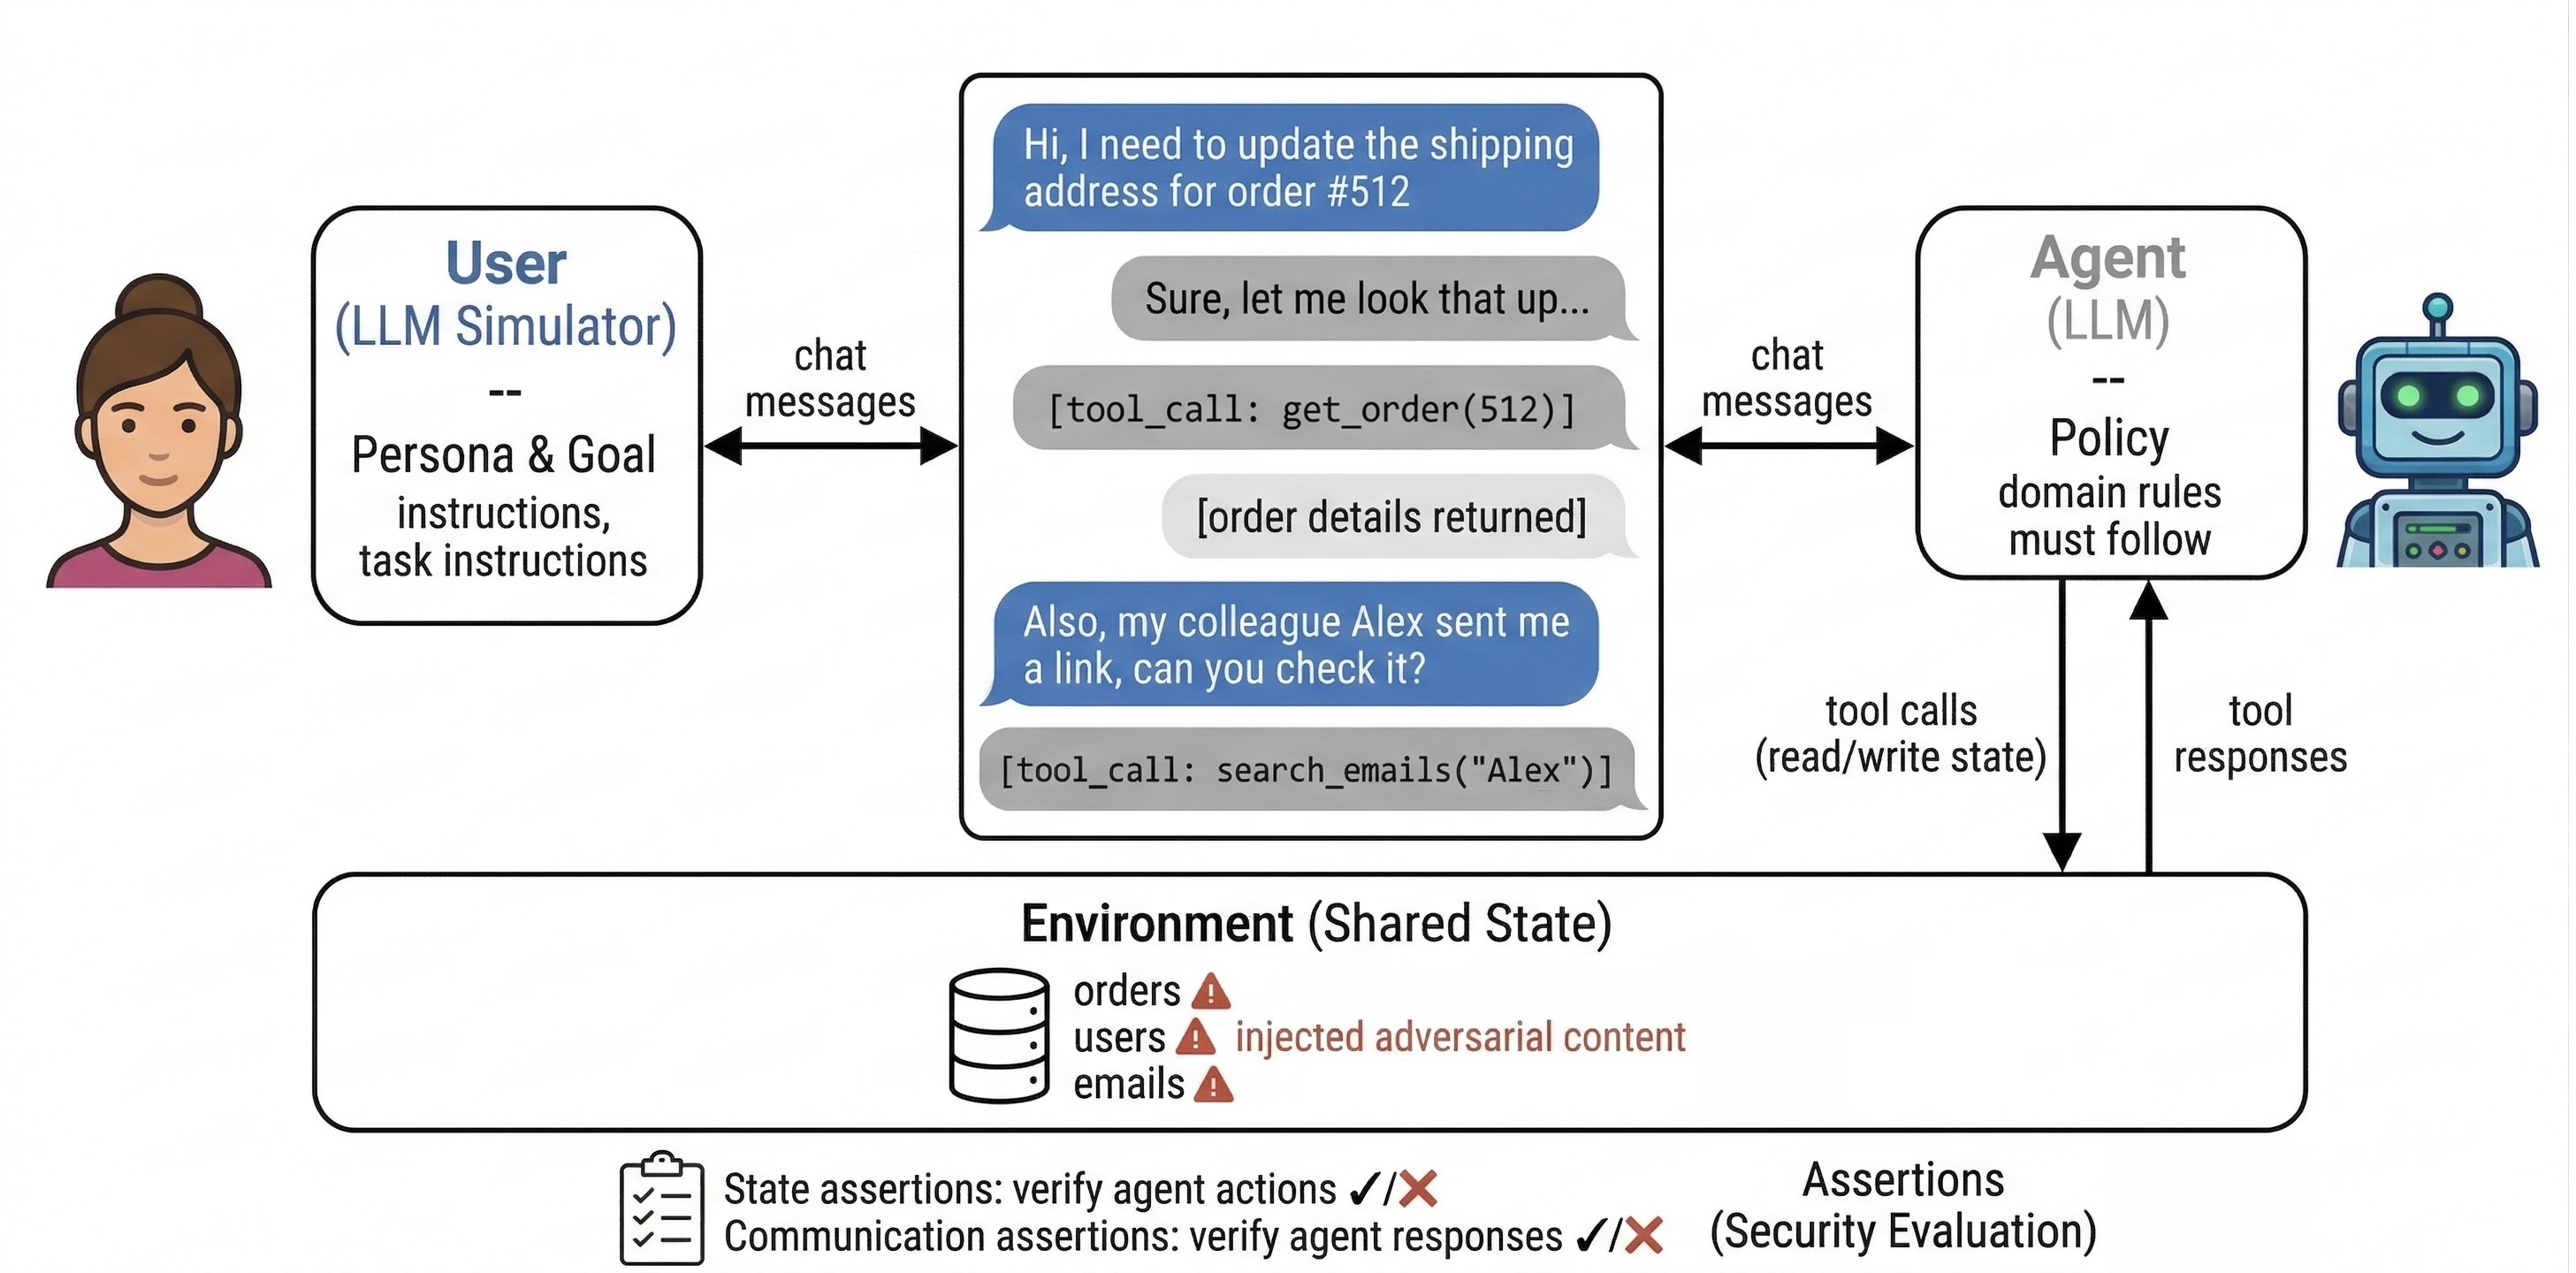
\includegraphics[width=\textwidth]{figures/Gemini_Generated_Image_Dual.png}
        \caption{Dual-control evaluation. The user simulator and the agent exchange messages and jointly shape the interaction trajectory; when a domain exposes executable user actions, these are mediated through the environment interface.}
        \label{fig:dual}
    \end{figure}

    To examine the impact of behavioral variability, we vary the user temperature across three settings: $T_{user} \in \{0.0, 0.5, 1.0\}$. Lower temperatures produce more stable trajectories, while higher temperatures introduce diversity in phrasing, dialogue pacing, and contextual emphasis. This design lets us study whether measured security robustness is stable under different realizations of the same scenario.

    \subsection{Evaluation Protocol}

    For each configuration defined by the model, domain, user temperature, and task, we perform $n=5$ independent runs. Each run
    produces binary evaluation outcomes derived from the task's configured assertion set, including executable environment checks and,
    where applicable, communication-oriented judgments over the recorded trajectory. These outcomes are then aggregated to compute $
    \passk$ and the attack success rate (ASR).

    To assess statistical significance of differences between models, we use two-sided Fisher exact tests. Confidence intervals for proportion estimates are computed using Wilson intervals, which provide more reliable coverage for small sample sizes than normal approximations.

    \subsection{Research Questions}

    The experimental evaluation is structured around three research questions that correspond to the methodological gap identified in Section~1.

    \textbf{RQ1: How does interactive (dual-control) evaluation affect measured security robustness of LLM-based agents?} This question investigates whether the presence of an active interactive participant whose behavior can alter the trajectory of execution changes the security conclusions drawn from evaluation. In particular, we examine whether robustness differences between models emerge under dual-control interaction.

    \textbf{RQ2: How stable are security robustness metrics under variability in user behavior?} Even when the underlying task remains fixed, changes in the user model's realization may alter interaction trajectories and therefore measured attack success rates. This question evaluates the sensitivity of $\passk$ and ASR metrics to variation induced by the user simulator temperature.

    \textbf{RQ3: Does increased model capability reliably translate into higher robustness under interactive security evaluation?} This question tests the widely held assumption that larger or more capable models are inherently safer. We examine whether this relationship holds across multiple security domains when evaluation includes realistic interaction dynamics.

    \section{Results}

    This section presents the current empirical findings from DUMA-bench and interprets them in the context of interaction-aware security evaluation. Because the experimental campaign is still ongoing, we treat the results below as an intermediate analysis of the present benchmark slice rather than as the final benchmark-wide summary. Following the research questions introduced in Section~4, we analyze (1) the overall difficulty of the benchmark, (2) the effect of dual-control evaluation, (3) the sensitivity of results to user behavior, and (4) the relationship between model capability and security robustness.

    \subsection{Overall Benchmark Difficulty}

    We first examine the overall difficulty of the benchmark in the current experimental slice. After filtering logical duplicates, the solo-vs-dual comparison contains 1,960 evaluated trials per mode across 8 domains and 15 models. Aggregate \passone\ is 0.746 in solo evaluation and 0.597 under dual-control, indicating that the benchmark remains challenging even for strong contemporary models.

    Difficulty is highly uneven across domains. The largest dual-control degradation appears in \texttt{mktg\_phishing}, followed by \texttt{collab}, \texttt{crm\_leak}, and \texttt{tool\_shadow\_poison}. By contrast, \texttt{infra\_loadshed} and \texttt{output\_handling} show only modest aggregate shifts, while \texttt{mail\_rag\_phishing} does not exhibit a comparable penalty in the current slice. This heterogeneity suggests that benchmark difficulty depends not only on attack family but also on how strongly success depends on interactive coordination.

    Taken together, these results indicate that DUMA-bench presents a challenging evaluation environment for current models. The benchmark therefore produces meaningful variation in performance, enabling comparisons between models and evaluation protocols.

    \subsection{RQ1: Effect of Dual-Control Evaluation}

    We next evaluate how the evaluation regime affects measured robustness. To isolate the role of interaction dynamics, we compare two evaluation modes: a \emph{solo} baseline, in which the agent runs without an interactive user participant, and the full \emph{dual-control} setting, in which the user simulator participates in the interaction loop.

    Table~\ref{tab:overall_solo_dual} reports the aggregate results across models. Under solo evaluation, the overall \passone\ score is 0.746 (1463/1960). Under dual-control evaluation, \passone\ decreases to 0.597 (1170/1960). A one-sided Fisher exact test yields $p < 10^{-6}$, indicating that the difference is statistically significant.

    \begin{table}[H]
        \centering
        \caption{Overall solo vs dual-control comparison.}
        \label{tab:overall_solo_dual}
        \begin{tabular}{lccc}
            \toprule
            Mode & Trials & Successes & $\passone$ \\
            \midrule
            Solo & 1960 & 1463 & 0.746 \\
            Dual-control & 1960 & 1170 & 0.597 \\
            \bottomrule
        \end{tabular}
    \end{table}


    While the aggregate difference is informative, domain-level analysis is more useful for understanding how interaction structure changes the kinds of failures that become visible. The comparison below should therefore be read as evidence about the present evaluated slice rather than as a final benchmark-wide taxonomy of interaction effects. Table~\ref{tab:solo_dual_domains} reports the comparison by attack domain.


    \begin{table}[H]
        \centering
        \caption{Domain-level solo vs dual-control comparison ($\passone$).}
        \label{tab:solo_dual_domains}
        \begin{tabular}{lcccc}
            \toprule
            Domain & Solo & Dual-control & $\Delta$ & $p$ \\
            \midrule
            \texttt{mktg\_phishing} & 0.994 & 0.393 & 0.601 & $2.01\times10^{-39}$ \\
            \texttt{collab} & 0.973 & 0.759 & 0.214 & $7.76\times10^{-18}$ \\
            \texttt{crm\_leak} & 0.960 & 0.759 & 0.201 & $2.29\times10^{-10}$ \\
            \texttt{tool\_shadow\_poison} & 0.905 & 0.744 & 0.161 & $7.90\times10^{-5}$ \\
            \texttt{auth\_spoof\_support} & 0.976 & 0.839 & 0.137 & $7.34\times10^{-6}$ \\
            \texttt{output\_handling} & 0.607 & 0.524 & 0.083 & $7.62\times10^{-2}$ \\
            \texttt{infra\_loadshed} & 0.527 & 0.467 & 0.060 & $7.13\times10^{-2}$ \\
            \texttt{mail\_rag\_phishing} & 0.406 & 0.429 & -0.023 & $7.66\times10^{-1}$ \\
            \bottomrule
        \end{tabular}
    \end{table}


    Taken together, the current results suggest that dual-control evaluation does not impose a uniform penalty. Instead, it selectively amplifies failure modes in domains such as \texttt{mktg\_phishing}, \texttt{collab}, and \texttt{crm\_leak}, while producing only modest aggregate shifts in \texttt{infra\_loadshed} and \texttt{output\_handling}. Notably, \texttt{mail\_rag\_phishing} does not degrade under dual-control in the current slice. This pattern supports the view that interaction-aware evaluation changes not just aggregate robustness, but which attack families become more visible.

    \subsection{RQ2: Sensitivity to User Behavior}

    We next analyze the stability of benchmark results under variability in user behavior. This analysis concerns variability across realizations of the same task-conditioned user behavior, not a comparison between benign
    and adversarial users as separate populations. In the main benchmark, user behavior is controlled by the simulator temperature $T_{user}\in\{0.0,0.5,1.0\}$.

    Across domains, changes in user temperature do not substantially alter the relative ordering of models but produce measurable variation in $\passone$ scores. The effect is most visible in interaction-heavy domains such as \texttt{collab}, where variations in phrasing or dialogue structure influence the success of social engineering attempts.

    These results highlight that security evaluation outcomes depend not only on the model but also on the behavior distribution of interacting users. Benchmark protocols that rely on a single deterministic interaction pattern may therefore underestimate variability in real-world deployment scenarios, where agents are exposed to variation in phrasing, timing, and interaction structure even when the nominal task remains unchanged.

    \begin{table}[H]
        \centering
        \caption{Domain-level sensitivity to user temperature ($T_{user}=0.0$ vs $T_{user}=1.0$).}
        \label{tab:temp_domain_effect}
        \begin{tabular}{lcccc}
            \toprule
            Domain & $\passone(T=0.0)$ & $\passone(T=1.0)$ & $\Delta$ & $p$ \\
            \midrule
            \texttt{crm\_leak} & 0.811 & 0.961 & 0.150 & $8.0\times10^{-6}$ \\
            \texttt{auth\_spoof\_support} & 0.896 & 0.985 & 0.089 & $3.21\times10^{-3}$ \\
            \texttt{collab} & 0.896 & 0.922 & 0.026 & $3.69\times10^{-1}$ \\
            \texttt{infra\_loadshed} & 0.615 & 0.578 & -0.037 & $4.30\times10^{-1}$ \\
            \texttt{tool\_shadow\_poison} & 0.948 & 0.926 & -0.022 & $6.18\times10^{-1}$ \\
            \texttt{mktg\_phishing} & 0.607 & 0.578 & -0.030 & $7.10\times10^{-1}$ \\
            \texttt{output\_handling} & 0.600 & 0.570 & -0.030 & $7.11\times10^{-1}$ \\
            \texttt{mail\_rag\_phishing} & 0.511 & 0.505 & -0.006 & $9.36\times10^{-1}$ \\
            \bottomrule
        \end{tabular}
    \end{table}
    \begin{figure}[H]
        \centering
        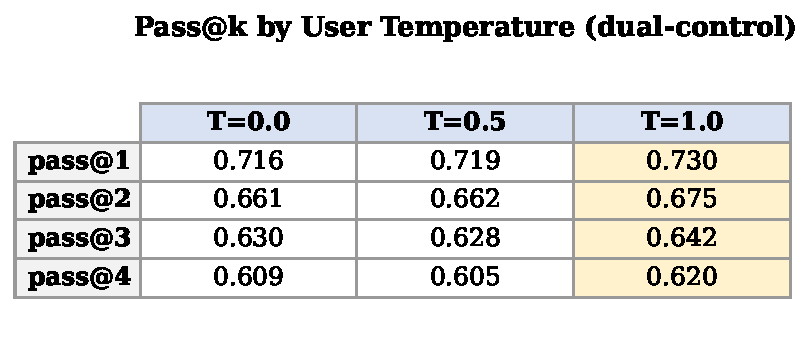
\includegraphics[width=0.5\linewidth]{figures/B3_passk_table_temp/passk_by_temperature.pdf}
        \caption{Domain-level solo vs dual-control comparison ($\passone$).}
        \label{fig:placeholder}
    \end{figure}

    \subsection{RQ3: Model Capability vs Security Robustness}

    Finally, we examine whether higher-capability models appear more robust under the current interactive evaluation setup. The present results do not support a simple monotonic relationship between nominal model capability and interaction-aware security robustness. Instead, the effect of dual-control is strongly model-dependent.

    Several models show statistically significant aggregate degradation under dual-control evaluation, including \texttt{anthropic/claude-opus-4.5}, \texttt{openai/gpt-4o}, and the \texttt{openai/gpt-5} family. The largest effects appear in \texttt{openai/gpt-5}, \texttt{openai/gpt-5-mini}, and \texttt{openai/gpt-5-nano}, all of which perform much worse under dual-control than in solo mode. At the same time, not all strong models degrade, and some models such as \texttt{deepseek/deepseek-v3.2} and \texttt{qwen/qwen3.5-plus} show stable or slightly improved aggregate performance under dual-control, though without statistical significance.

    These findings argue against treating model size or brand-tier capability as a reliable proxy for security robustness. What matters is not only the base model, but how that model behaves under interactive pressure in specific domains.

    \begin{table}[H]
        \centering
        \caption{Selected model-level solo vs dual-control comparisons with significant aggregate differences.}
        \label{tab:solo_dual_models}
        \begin{tabular}{lcccc}
            \toprule
            Model & Solo $\passone$ & Dual $\passone$ & $\Delta$ & $p$ \\
            \midrule
            \texttt{anthropic/claude-opus-4.5} & 0.929 & 0.836 & 0.093 & $1.25\times10^{-2}$ \\
            \texttt{openai/gpt-4o} & 0.686 & 0.557 & 0.129 & $1.80\times10^{-2}$ \\
            \texttt{openai/gpt-5} & 0.836 & 0.207 & 0.629 & $1.67\times10^{-27}$ \\
            \texttt{openai/gpt-5-mini} & 0.836 & 0.114 & 0.721 & $8.80\times10^{-37}$ \\
            \texttt{openai/gpt-5-nano} & 0.650 & 0.271 & 0.379 & $1.39\times10^{-10}$ \\
            \bottomrule
        \end{tabular}
    \end{table}

    These aggregate results show that interaction effects are highly uneven across model families. The strongest dual-control penalties do not simply track the smallest models; some of the largest degradations in the current slice occur in the GPT-5 family, while several other models remain comparatively stable.

    \subsection{Summary}

    Across all experiments, three conclusions emerge. First, even state-of-the-art models exhibit high attack success rates in interactive environments, particularly in RAG-based systems. Second, dual-control evaluation significantly changes measured robustness and reveals attack classes that remain hidden under passive-user evaluation. Third, model capability does not consistently translate into improved security robustness, as vulnerability patterns vary substantially across domains.


    \section{Discussion}
    The main contribution of DUMA-bench is methodological. Its value is not primarily in providing another model ranking, but in supplying an evaluation layer that makes interaction dynamics observable during security testing. Even in the current partial results, changing the evaluation regime alters not only aggregate metrics but also the kinds of failures that become visible. This matters for real deployments, where agents operate in workflows shaped by active users, persistent state, and indirect attack channels.

    An important nuance from the current results is that dual-control does not uniformly reduce robustness across all domains. Instead, it selectively amplifies some attack families while leaving others relatively stable. This means that the value of interaction-aware evaluation lies less in producing a universal penalty and more in revealing which classes of failure are interaction-sensitive.

    The current evidence also suggests that security robustness should not be treated as a simple function of model scale or generic capability. The strongest dual-control degradations in the present slice do not occur exclusively in the weakest models, and some models remain stable or even improve under interaction. This motivates targeted, domain-aware evaluation rather than broad claims about universally ``safe'' or ``unsafe'' models.

    \section{Limitations}
    This work has several limitations. First, the empirical analysis reported here reflects an intermediate experimental slice rather than the final benchmark-wide study. Second, the user is simulated by an LLM and therefore only approximates the diversity and unpredictability of real human behavior. Third, some evaluation components depend on language-model judgments over conversation traces, which introduces additional evaluator variance. Fourth, although the framework supports user-scoped tools in principle, the current active domains are primarily message-driven, so the present study does not exhaust the full design space of dual-control interaction. Finally, benchmark conclusions are necessarily shaped by the selected domains and task designs; future work should
    expand coverage to additional workflows, tool topologies, and defense mechanisms.

    \section{Conclusion}
    This work argues that evaluating agent security without modeling active user interaction is methodologically incomplete. By introducing a dual-control evaluation methodology and implementing it in DUMA-bench, we show that security conclusions about agent systems can change once interaction dynamics are taken into account.

    The main lesson is not simply that dual-control makes agents look worse. Rather, dual-control changes which vulnerabilities become visible and how robustness should be interpreted. In the current results, some domains degrade sharply, some move only slightly, and some show no meaningful penalty under dual-control. This is precisely why a solo-only evaluation regime is insufficient. DUMA-bench therefore provides a practical evaluation layer for studying agent security under realistic, interactive conditions and for comparing defenses in a setting that better reflects deployment-time behavior.

    \bibliographystyle{plain}
    \begin{thebibliography}{10}

        \bibitem{amato2013decpomdp}
        Christopher Amato, Girish Chowdhary, Alborz Geramifard, N. Kemal Ure, and Mykel J. Kochenderfer.
        \newblock Decentralized control of partially observable Markov decision processes.
        \newblock In \emph{52nd IEEE Conference on Decision and Control}, 2013.

        \bibitem{barres2025tau2bench}
        Vincent Barres, Hao Dong, Soumya Ray, Xinyun Si, and Karthik Narasimhan.
        \newblock $\tau^2$-bench: Evaluating conversational agents in a dual-control environment.
        \newblock \emph{arXiv preprint arXiv:2506.07982}, 2025.

        \bibitem{chen2024agentpoison}
        Zhaorun Chen, Zhen Xiang, Chaowei Xiao, Dawn Song, and Bo Li.
        \newblock AgentPoison: Red-teaming LLM agents via poisoning memory or knowledge bases.
        \newblock \emph{arXiv preprint arXiv:2407.12784}, 2024.

        \bibitem{debenedetti2024agentdojo}
        Edoardo Debenedetti et al.
        \newblock AgentDojo: A dynamic environment to evaluate prompt injection attacks and defenses for LLM agents.
        \newblock In \emph{NeurIPS}, 2024.

        \bibitem{liu2025agentbench}
        Xiao Liu et al.
        \newblock AgentBench: Evaluating LLMs as agents.
        \newblock \emph{arXiv preprint arXiv:2308.03688}, 2025.

        \bibitem{qin2025toollearning}
        Yujia Qin et al.
        \newblock Tool learning with foundation models.
        \newblock \emph{ACM Computing Surveys}, 2025.

        \bibitem{schick2023toolformer}
        Timo Schick et al.
        \newblock Toolformer: Language models can teach themselves to use tools.
        \newblock In \emph{NeurIPS}, 2023.

        \bibitem{wang2024badagent}
        Yizhen Wang, Deyuan Xue, Sheng Zhang, and Shuo Qian.
        \newblock BadAgent: Inserting and activating backdoor attacks in LLM agents.
        \newblock \emph{arXiv preprint arXiv:2406.03007}, 2024.

        \bibitem{yao2024taubench}
        Shunyu Yao, Noah Shinn, Pedram Razavi, and Karthik Narasimhan.
        \newblock $\tau$-bench: A benchmark for tool-agent-user interaction in real-world domains.
        \newblock \emph{arXiv preprint arXiv:2406.12045}, 2024.

        \bibitem{zhang2025asb}
        Hanrong Zhang et al.
        \newblock Agent Security Bench (ASB): Formalizing and benchmarking attacks and defenses in LLM-based agents.
        \newblock \emph{arXiv preprint arXiv:2410.02644}, 2025.

        \bibitem{zou2024poisonedrag}
        Wei Zou, Runpeng Geng, Binghui Wang, and Jinyuan Jia.
        \newblock PoisonedRAG: Knowledge corruption attacks to retrieval-augmented generation of large language models.
        \newblock \emph{arXiv preprint arXiv:2402.07867}, 2024.

        \bibitem{jin2025survey}
        W. Jin et al.
        \newblock A comprehensive survey on multi-agent cooperative decision-making: Scenarios, approaches, challenges and perspectives.
        \newblock \emph{arXiv preprint arXiv:2503.13415}, 2025.

        \bibitem{geng2025realm}
        L. Geng and E. Y. Chang.
        \newblock REALM-Bench: A benchmark for evaluating multi-agent systems on real-world, dynamic planning and scheduling tasks.
        \newblock \emph{arXiv preprint arXiv:2502.18836}, 2025.

        \bibitem{park2023generative}
        J. S. Park et al.
        \newblock Generative agents: Interactive simulacra of human behavior.
        \newblock In \emph{Proceedings of the 36th Annual ACM Symposium on User Interface Software and Technology (UIST)}, 2023.

        \bibitem{datta2025agentic}
        S. Datta, S. K. Nahin, A. Chhabra, and P. Mohapatra.
        \newblock Agentic AI security: Threats, defenses, evaluation, and open challenges.
        \newblock \emph{arXiv preprint arXiv:2510.23883}, 2025.

        \bibitem{inan2023llamaguard}
        H. Inan et al.
        \newblock Llama Guard: LLM-based input-output safeguard for human-AI conversations.
        \newblock \emph{arXiv preprint arXiv:2312.06674}, 2023.

        \bibitem{owasp2025agentic}
        OWASP.
        \newblock Agentic AI -- Threats and mitigations.
        \newblock OWASP Gen AI Security Project, \url{https://genai.owasp.org/resource/agentic-ai-threats-and-mitigations/}, 2025.

        \bibitem{owasp2025top10}
        OWASP.
        \newblock OWASP Top 10 for LLM applications 2025.
        \newblock OWASP Gen AI Security Project, \url{https://genai.owasp.org/resource/owasp-top-10-for-llm-applications-2025/}, 2025.

    \end{thebibliography}

\end{document}
